\chapter{Panoptic Quality}\label{ch:metric}

\section{Introduction}\label{sec:metric-intro}
\epigraph{When you can measure what you are speaking about, and express it in numbers, you know
something about it.}{Lord Kelvin, in a lecture of 3 May 1883, printed in \citet{kelvin1889}}

The competition scores every submission with a single number, the \keyterm{Panoptic Quality}
(PQ). The metric was introduced by \citet{pq} for panoptic segmentation, and the competition uses
its instance-segmentation form.\footnote{\citet{pq} proposed panoptic segmentation as a single
task that unifies semantic segmentation (``stuff'') and instance segmentation (``things''), and
designed PQ to score both kinds of region with one formula.} Since every result in this book is a PQ number, it pays to
understand the metric thoroughly: what it rewards, what it punishes, and how much each kind of
mistake costs. In Section~\ref{sec:metric-matching} we define how predictions are matched to
annotations, and in Section~\ref{sec:metric-sqrq} we split PQ into two factors that measure
delineation and detection separately. Section~\ref{sec:metric-pooling} explains how the counts
from different annotators are combined. Section~\ref{sec:metric-leverage} works out how much each
kind of change to a submission is worth, a calculation we will use throughout the book.
Sections~\ref{sec:metric-agreement} and~\ref{sec:metric-uncertainty} ask how well human annotators
agree with each other, and how precisely a PQ value measured on a finite validation set can be
trusted. Finally, Section~\ref{sec:metric-code} compares the organisers' implementation of the
metric with ours.

\section{Matching predictions to annotations}\label{sec:metric-matching}
Consider one photograph, one annotator's record of it, and the set of masks that a model predicted
for that photograph. The first step of the metric pairs predictions with annotations. A predicted
mask $p$ and an annotated mask $g$ \keyterm{match} when
\begin{equation}
\IoU(p,g)=\frac{|p\cap g|}{|p\cup g|}>\tfrac12 .
\end{equation}
Matched pairs are called \keyterm{true positives}. A prediction that matches no annotation is a
\keyterm{false positive}, and an annotation that matches no prediction is a \keyterm{false
negative}.

It is not obvious that this rule defines a proper matching. Could one annotation match two
predictions, so that it would be counted twice? The following result shows that it cannot,
provided that the predictions do not overlap each other, which the competition requires.

\begin{theorem}[matches above an IoU of one half are unique]\label{thm:metric-unique}
If the predicted masks are pairwise disjoint, then each annotation matches at most one prediction.
Likewise, since the annotated masks of one record are pairwise disjoint, each prediction matches at
most one annotation.
\end{theorem}
\begin{proof}
If $\IoU(p,g)>\tfrac12$, then $|p\cap g|>\tfrac12|p\cup g|\ge\tfrac12|g|$, so a prediction that
matches $g$ covers more than half of $g$. If two disjoint predictions $p_1$ and $p_2$ both matched
$g$, then $p_1\cap g$ and $p_2\cap g$ would be disjoint subsets of $g$, each containing more than
half of its pixels, which is impossible. The second statement follows by exchanging the roles of
predictions and annotations.
\end{proof}

Theorem~\ref{thm:metric-unique} has a useful practical consequence. The organisers' notebook marks
\emph{every} pair above the threshold as a true positive, whereas our own evaluator performs a
greedy one-to-one matching in order of decreasing IoU. For disjoint masks the two procedures produce
the same pairs, so there is no need for an optimal assignment algorithm such as the Hungarian
method~\citep{kuhn,munkres1957}, and the two
implementations agree (Section~\ref{sec:metric-code}).

\section{Segmentation quality and recognition quality}\label{sec:metric-sqrq}
Given the matches, Panoptic Quality is defined as
\begin{equation}
\PQ=\frac{\sum_{(p,g)\in\TP}\IoU(p,g)}{|\TP|+\tfrac12|\FP|+\tfrac12|\FN|}.
\label{eq:metric-pq}
\end{equation}
The numerator rewards each true positive by the quality of its mask. The denominator counts every
true positive once and charges half a unit for every false positive and every false negative.
Multiplying and dividing by $|\TP|$ splits PQ into two factors with separate meanings:
\begin{equation}
\PQ=\underbrace{\frac{1}{|\TP|}\sum_{(p,g)\in\TP}\IoU(p,g)}_{\textstyle\SQ}
\;\times\;
\underbrace{\frac{|\TP|}{|\TP|+\tfrac12|\FP|+\tfrac12|\FN|}}_{\textstyle\RQ}.
\label{eq:metric-sqrq}
\end{equation}
The \keyterm{segmentation quality} (SQ) is the mean IoU of the matched pairs, so it measures how
well the filaments that were found have been outlined. The \keyterm{recognition quality} (RQ)
measures detection. In fact RQ is the familiar $F_1$ score~\citep{vanrijsbergen1979} of detection at an IoU threshold of one
half. With precision $|\TP|/(|\TP|+|\FP|)$ and recall $|\TP|/(|\TP|+|\FN|)$, we have
\begin{equation}
F_1=\frac{2\,\mathrm{precision}\cdot\mathrm{recall}}{\mathrm{precision}+\mathrm{recall}}
    =\frac{2|\TP|}{2|\TP|+|\FP|+|\FN|}=\RQ .
\end{equation}

\subsection{Example: scoring one record by hand}\label{sec:metric-example}
Suppose that an annotator drew four filaments $g_1,\dots,g_4$ on a photograph, and that the model
predicted four disjoint masks $p_1,\dots,p_4$. Suppose further that $\IoU(p_1,g_1)=0.80$,
$\IoU(p_2,g_2)=0.60$ and $\IoU(p_3,g_3)=0.45$, that $p_4$ overlaps no annotation, and that nothing
was predicted near $g_4$. The first two pairs match. The third does not, because its IoU is below
one half, so $p_3$ counts as a false positive and $g_3$ as a false negative. In total we have two
true positives, two false positives ($p_3$ and $p_4$) and two false negatives ($g_3$ and $g_4$).
Hence
\begin{gather*}
\SQ=\frac{0.80+0.60}{2}=0.70,\qquad
\RQ=\frac{2}{2+\tfrac12\cdot2+\tfrac12\cdot2}=0.50,\\
\PQ=\SQ\times\RQ=0.35 .
\end{gather*}
Now suppose that a better model draws $p_3$ slightly more accurately, so that its IoU with $g_3$
rises from 0.45 to 0.55. The pair now matches, and we have three true positives, one false
positive and one false negative. The numerator becomes $0.80+0.60+0.55=1.95$, the denominator
becomes $3+\tfrac12+\tfrac12=4$, and PQ rises from 0.35 to about 0.49. A small improvement to a
single mask has raised the score of the whole record by almost 40\%, because it moved a prediction across
the threshold of one half. We will see in Section~\ref{sec:metric-leverage} that this asymmetry is
a general property of the metric.

\subsection{Two properties of SQ}\label{sec:metric-sq-properties}
Two properties of SQ are easy to forget, and both caused real mistakes during the project. First,
SQ is an average over matched pairs only, and every matched pair has an IoU above one half by
construction. Consequently SQ can never fall below 0.5, and it says nothing about the filaments
that were missed. If we compare the SQ of one method with the mean per-instance IoU of another
method computed over \emph{all} instances, we compare a filtered population with an unfiltered one.
We made exactly this comparison in one analysis (exp129) and had to retract it. Second, SQ and RQ
interact. A change that finds additional faint filaments usually adds matches with fairly low IoU,
which can lower SQ even as it raises RQ and PQ.

\section{Pooling over annotation records}\label{sec:metric-pooling}
The competition does not compute PQ for each photograph and then average the results. Instead it
\keyterm{pools} the counts over every \emph{annotation record} $r$ and divides once:
\begin{equation}
\PQ=\frac{\sum_r\sum_{(p,g)\in\TP_r}\IoU(p,g)}{\sum_r\bigl(|\TP_r|+\tfrac12|\FP_r|+\tfrac12|\FN_r|\bigr)}.
\label{eq:metric-pooled}
\end{equation}
This has three consequences. First, a photograph with three annotators counts three times, because
the model's single set of predictions is scored separately against each annotator. Second, the
same prediction can be right and wrong at once: a mask can match a filament that annotator A drew
and be a false positive for annotator B, who did not draw it. Third, crowded photographs carry more
weight than sparse ones, since a photograph with twenty filaments contributes much more to the
denominator than a photograph with two. One advantage of pooling is that a nearly empty photograph
cannot swing the result, as it could if we averaged per-photograph scores.

Pooling also makes it important to state the unit of every count. The validation split described
in Chapter~\ref{ch:validation} contains 106 photographs but 180 records, so a count made per
photograph and a count made per record differ by a factor of about $180/106\approx1.7$. In one
analysis (exp121) we counted admitted candidates per photograph, but true and false positives per
record. The mismatch produced an apparent ``fragmentation'' effect that took an hour to explain.

\section{What each kind of change is worth}\label{sec:metric-leverage}
We now ask how much each kind of change to a submission is worth. Write $S=\sum_{\TP}\IoU$ for the
numerator of Equation~\eqref{eq:metric-pq} and $D=|\TP|+\frac12|\FP|+\frac12|\FN|$ for its
denominator, so that $\PQ=S/D$. For the final model on the validation split we have
$|\TP|=\NumTP{}$, $|\FP|=\NumFP{}$, $|\FN|=\NumFN{}$ and $\SQ=\ValSQ{}$, so that $S\approx604$,
$D=1283.5$ and $\PQ=\HostPQ{}$. Each kind of change moves $S$ and $D$ in a characteristic way.

\paragraph{Adding a false positive.} The denominator grows by $\tfrac12$ and the numerator is
unchanged, so
\begin{equation}
\Delta\PQ=\frac{S}{D+\frac12}-\frac{S}{D}\approx-\frac{\PQ}{2D}.
\end{equation}

\paragraph{Finding a missed filament} with a mask of IoU $q$. One false negative becomes a true
positive. The numerator gains $q$, and the denominator gains 1 for the new true positive and loses
$\tfrac12$ for the false negative that disappears, a net change of $+\tfrac12$. The score rises if
and only if
\begin{equation}
\frac{S+q}{D+\frac12}>\frac{S}{D}\iff q>\tfrac12\PQ,
\end{equation}
which always holds, because a match requires $q>\tfrac12$ and $\PQ<1$.

\paragraph{Rescuing a near miss.} Suppose that a prediction overlaps its filament with an IoU of
0.49. It then counts as both a false positive and a false negative. If we improve it until the IoU
is 0.51, the pair becomes one true positive. The denominator changes by $+1-\tfrac12-\tfrac12=0$,
and the numerator gains 0.51. By comparison, improving an existing match from an IoU of 0.55 to
0.60 adds only 0.05 to the numerator. Moving a prediction across the threshold is therefore worth
about ten times as much as a comparable improvement to a mask that already matches. This asymmetry,
which we saw in the example of Section~\ref{sec:metric-example}, explains why we spent so much
effort on predictions that fall just below the threshold (Chapter~\ref{ch:post}).

Figure~\ref{fig:metric-leverage} shows the three effects, starting from the deployed model's
counts. Recovering fifty missed filaments at an IoU of 0.65 would raise PQ to
\LeverageRecover{}; removing fifty false positives would raise it to \LeverageRemove{}; and
improving fifty existing matches by 0.05 IoU each would raise it only to \LeveragePolish{}.

\begin{figure}[t]
\centering
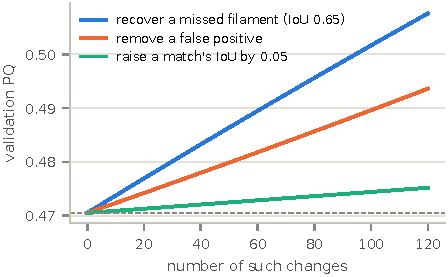
\includegraphics[width=0.66\textwidth]{figures/fig_leverage.pdf}
\caption{Validation PQ after $n$ changes of each kind, starting from the deployed model. Recovering
a missed filament is worth more than removing a false positive, and both are worth far more than
improving matches that already exist. \generatedby{book/make\_book\_figures.py:fig\_leverage}}
\label{fig:metric-leverage}
\end{figure}

\subsection{Why tuning a threshold rarely helps}\label{sec:metric-threshold}
Every model in this book outputs candidate masks with confidence scores, and a threshold decides
which candidates to keep. Lowering the threshold admits more candidates. Some of them become true
positives with a mean IoU of $q$, and the rest become false positives. If we admit $k$ correct and
$m$ incorrect candidates, the score changes to $(S+kq)/(D+\tfrac12k+\tfrac12m)$, which exceeds
$S/D$ if and only if
\begin{equation}
\frac{k}{k+m}>\frac{\PQ}{2q}.
\label{eq:metric-breakeven}
\end{equation}
In words, the precision of the newly admitted candidates must exceed $\PQ/(2q)$. With
$\PQ\approx0.46$ and $q\approx0.65$ this is about 35\%. At the optimal threshold, the
\emph{marginal} candidates sit at this break-even precision, so small moves of the threshold in
either direction change the score very little. In other words, PQ is flat near its optimum as a
function of the threshold. For example, in exp002 we swept seven thresholds and three minimum
areas, and the best setting in the whole grid was only $0.0022$ better than the default. We return
to Equation~\eqref{eq:metric-breakeven} in Chapter~\ref{ch:recall}, where it decides whether any
method for rescuing discarded candidates can possibly raise the score.

\section{How well do annotators agree?}\label{sec:metric-agreement}
The metric compares a model with the judgement of one person. How well do two people agree under
the same rule? We can measure this by treating one annotator's masks as ``predictions'' and scoring
them against another annotator's masks on the same photograph, for every ordered pair of
annotators. Over all 296 photographs with more than one annotator (\HumanPairs{} ordered pairs),
the result is $\PQ=\HumanPQAll{}$. On the validation photographs it is $\PQ=\HumanPQ{}$, with
$\SQ=\HumanSQ{}$ and $\RQ=\HumanRQ{}$
(\file{experiments/exp\_145\_host\_evaluation/src/annotator\_agreement.py}).

The final model scores \HostPQ{} against the same annotators, well above this value. Two
interpretations of this comparison are tempting, and both are wrong. The first is that the model is
better than the experts. It is not: a model trained on the labels of many annotators learns
something like their average, and an average lies closer to each individual than two individuals
lie to each other. This is a form of regression to the mean, and it does not indicate superhuman
skill. The second is that \HumanPQAll{} is a ceiling, so that nothing more can be gained. This is
also false. Each test photograph is scored against the annotator who labelled it, and a model can
match any single annotator better than another annotator does. The agreement between annotators
measures how uncertain the labels are; it does not bound the score.

A further experiment clarified the nature of the disagreement. If annotators were noisy
measurements of a single true outline, then combining two of them should predict a third better
than either one does alone, just as averaging several noisy measurements reduces their
error~\citep{galton1907}. On
the 151 photographs with three annotators, a consensus of two annotators predicted the held-out
third with a PQ of 0.3291, while a single other annotator did so with 0.3287. The consensus helped
by only 0.0004. The disagreement therefore appears to be \emph{structured}: annotators make
different decisions about where a faint extension stops belonging to a filament, and about whether
two nearby patches form one object or two. Such differences of judgement do not scatter at
random around a hidden true answer, so averaging does not remove them. The standard statistical
models of annotators, from the error-rate model of \citet{dawid1979} to STAPLE~\citep{warfield2004}
and the learning-from-crowds model of \citet{raykar2010}, assume a hidden true label of this kind.
Our measurement does not test those models directly, but it suggests that their central assumption
fits these labels poorly.

\section{How certain is a score?}\label{sec:metric-uncertainty}
A validation PQ of 0.4705 is a measurement on 106 photographs, and a different set of 106
photographs would have given a different value. The \keyterm{bootstrap}~\citep{efron1979,bootstrap} estimates
how different. We draw 106 photographs \emph{with replacement} from the validation set, recompute
the pooled PQ on this resampled set, and repeat the procedure 10,000 times. The spread of the
recomputed values approximates the sampling distribution of the score, and its 2.5th and 97.5th
percentiles form a 95\% \keyterm{percentile interval}.

The resampling unit must be the photograph and not the record. The records of one photograph share
a single set of predictions, so they are not independent, and resampling them separately would
pretend that the data contain more independent evidence than they do. Listing~\ref{lst:metric-bootstrap}
first sums the counts of each photograph and then resamples these sums.

\begin{lstlisting}[caption={Photograph-level bootstrap of pooled PQ. From \file{paper/make\_figures.py:bootstrap}.},label=lst:metric-bootstrap]
def pooled(sums):   # sums[..., :] = (sum of TP IoU, TP, FP, FN)
    iou, tp, fp, fn = sums[..., 0], sums[..., 1], sums[..., 2], sums[..., 3]
    denominator = tp + 0.5 * fp + 0.5 * fn
    return iou / denominator, iou / np.maximum(tp, 1), tp / denominator

def bootstrap(per_photo, draws=10000, seed=2026):
    rng = np.random.default_rng(seed)
    picks = rng.integers(0, len(per_photo), size=(draws, len(per_photo)))
    pq, sq, rq = pooled(per_photo[picks].sum(axis=1))
    return np.percentile(pq, [2.5, 97.5])
\end{lstlisting}

Figure~\ref{fig:metric-bootstrap} shows the result. The model's interval is \PQLow{}--\PQHigh{},
and the annotators' interval is \HumanPQLow{}--\HumanPQHigh{}, so the two do not overlap. The
model's interval is about 0.04 wide. This is a large number compared with the effects we usually
measured: most of the individual changes tested in this book moved validation PQ by less than 0.01,
well inside the interval. We dealt with this in two ways. We compared variants of a model on the
\emph{same} photographs, since most of the variation from photograph to photograph then cancels
out (Exercise~\ref{ex:metric-paired} makes this precise), and we treated small differences as noise
unless such a paired comparison showed otherwise.

\begin{figure}[t]
\centering
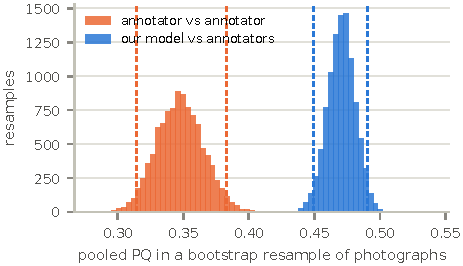
\includegraphics[width=0.66\textwidth]{figures/fig_bootstrap.pdf}
\caption{Bootstrap distributions of pooled PQ over 10,000 resamples of the validation photographs,
for the deployed model and for the agreement between annotators. Dashed lines mark the 95\%
percentile intervals. \generatedby{book/make\_book\_figures.py:fig\_bootstrap}}
\label{fig:metric-bootstrap}
\end{figure}

For a rate, such as the recall of filaments within a range of sizes, we use the \keyterm{Wilson
score interval}~\citep{wilson}. For $k$ successes in $n$ trials, with $\hat p=k/n$ and $z=1.96$, it
is
\begin{equation}
\frac{\hat p+\frac{z^2}{2n}}{1+\frac{z^2}{n}}\pm
\frac{z}{1+\frac{z^2}{n}}\sqrt{\frac{\hat p(1-\hat p)}{n}+\frac{z^2}{4n^2}} .
\end{equation}
Unlike the textbook interval $\hat p\pm z\sqrt{\hat p(1-\hat p)/n}$, the Wilson interval always
stays inside $[0,1]$ and behaves well when $n$ is small~\citep{agresti1998}.

\section{The organisers' implementation and ours}\label{sec:metric-code}
The organisers publish a self-evaluation notebook that contains their scoring code.
Listing~\ref{lst:metric-host} shows its core, and Listing~\ref{lst:metric-ours} shows our own
implementation. On the final model's validation predictions, the two return 0.4705249989 and
0.4705249990 respectively, with identical counts of true positives, false positives and false
negatives (exp145). They agree to nine decimal places.

\begin{lstlisting}[caption={The organisers' PQ, from their self-evaluation notebook (\file{experiments/exp\_145\_host\_evaluation/host/self\_evaluation\_notebook.ipynb}), lightly condensed.},label=lst:metric-host]
def get_pq_score(overlap_df):
    tp_iou_scores, fp_count, fn_count = [], 0, 0
    for row in overlap_df.itertuples(index=False):   # one row per annotator-image
        if row.n_gt == 0:
            fp_count += row.n_pred; continue
        if row.n_pred == 0:
            fn_count += row.n_gt; continue
        hit_matrix = row.iou_matrix > 0.5            # every pair above the threshold
        tp_iou_scores.extend(row.iou_matrix[hit_matrix].tolist())
        fp_count += int((hit_matrix.sum(dim=0) == 0).sum())   # predictions hitting nothing
        fn_count += int((hit_matrix.sum(dim=1) == 0).sum())   # annotations hit by nothing
    denominator = len(tp_iou_scores) + 0.5 * fp_count + 0.5 * fn_count
    return sum(tp_iou_scores) / denominator if denominator > 0 else 0.0
\end{lstlisting}

\begin{lstlisting}[caption={Our PQ for one record, and the pooling over records. Condensed from \file{shared/utils.py:compute\_pq} and \file{aggregate\_pq}.},label=lst:metric-ours]
def compute_pq(pred_masks, gt_masks, iou_threshold=0.5):
    ious = mask_util.iou(pred_rles, gt_rles, [0] * len(gt_rles))   # on RLE, in C
    matched_pred, matched_gt, iou_sum = set(), set(), 0.0
    pairs = np.argwhere(ious > iou_threshold)
    for i, j in sorted(pairs, key=lambda p: -ious[p[0], p[1]]):   # greedy, best first
        if i in matched_pred or j in matched_gt:
            continue
        matched_pred.add(i); matched_gt.add(j); iou_sum += ious[i, j]
    tp = len(matched_pred)
    return dict(tp=tp, fp=len(pred_masks) - tp, fn=len(gt_masks) - tp, iou_sum=iou_sum)

def aggregate_pq(per_record):
    tp = sum(r["tp"] for r in per_record); fp = sum(r["fp"] for r in per_record)
    fn = sum(r["fn"] for r in per_record); iou_sum = sum(r["iou_sum"] for r in per_record)
    return iou_sum / (tp + 0.5 * fp + 0.5 * fn)
\end{lstlisting}

There is one situation in which the two implementations disagree: two \emph{identical}
predictions placed over one annotation. The organisers' code counts two true positives, whereas ours
counts one true positive and one false positive. This case violates the premise of
Theorem~\ref{thm:metric-unique}, and since the scorer rejects overlapping submissions it can never
reach the leaderboard. We nevertheless pin it with a dedicated test
(\file{tests/test\_pq\_matches\_official.py}), so that the assumption remains visible to anyone who
changes the code.

\section*{Exercises}
\begin{exercise}{Uniqueness}
Construct two predictions that overlap each other and that both match the same annotation with an
IoU above one half. Which step in the proof of Theorem~\ref{thm:metric-unique} fails?
\end{exercise}

\begin{exercise}{RQ is $F_1$}
Show that RQ in Equation~\eqref{eq:metric-sqrq} equals the $F_1$ score of detection, and that
$\SQ\ge\tfrac12$ whenever $|\TP|>0$.
\end{exercise}

\begin{exercise}{Break-even precision}
Derive Equation~\eqref{eq:metric-breakeven}. Then show that when a model's threshold is optimal,
the precision of the marginal candidates equals $\PQ/(2q)$. What does this imply about the shape of
PQ as a function of the threshold near its maximum?
\end{exercise}

\begin{exercise}{Pooling versus averaging}
Using the final model's counts per record (recompute them with
\file{paper/make\_figures.py:record\_sums}), compare the pooled PQ with the mean of the per-record
PQ values and with the mean of the per-photograph PQ values. Which photographs cause the
differences?
\end{exercise}

\begin{exercise}{A paired bootstrap}\label{ex:metric-paired}
Suppose two models are scored on the same 106 photographs. Adapt Listing~\ref{lst:metric-bootstrap}
to bootstrap the \emph{difference} between their PQ values, resampling the photographs jointly for
both models. Show that the interval for the difference is much narrower than one would infer from
the two separate intervals, and explain why.
\end{exercise}
